% =====================================================================
% SKELETON ONLY. Every rendered word is Lorem Ipsum; every instruction
% is a % comment, so nothing here can leak into the finished paper.
%
%   pdflatex skeleton && pdflatex skeleton
%
% PAGE BUDGET (target -> what belongs there)
%   1.0  abstract ~200 words w/ three numbers; intro ~600 words; teaser figure
%   1.0  related work ~250 words; Sec IV-A; Prop 1; Prop 2 + two-line proof
%   1.2  benchmark, protocol, Table 1 floors/ceilings, paired bootstrap
%   1.3  scaling figure + merged mechanism table + second figure
%   1.2  the two controls: query-conditioned encoder, then local geometry
%   0.8  replications merged into one table; r and Corollary 5 compressed
%   0.8  limitations and conclusion
%   0.7  references
%   ---
%   8.0  total
%
% Replace \filler{n} with real prose. One placeholder paragraph is ~50 words and
% ~0.055 of a text page, so \filler{n} reserves roughly 50n words.
%
% NOTE ON THE TWO SETS OF NUMBERS. The word counts in the per-section comments
% are the MINIMUM each slot needs to make its argument; they total ~2600 words
% and fill about five pages once the floats are placed. The \filler{n} calls are
% sized to fill the eight-page budget above, ~4700 words. The difference is
% headroom: either the paper is comfortably shorter than budgeted, or those
% sections can say more than the minimum. Decide that per section rather than
% globally, and shrink the \filler back as real prose replaces it.
%
% Check as you go with:   texcount -inc -sum skeleton.tex
% =====================================================================

\documentclass[10pt,twocolumn,letterpaper]{article}

\usepackage[margin=0.75in,columnsep=0.25in]{geometry}
\IfFileExists{ptmr7t.tfm}{\usepackage{times}}{}
\usepackage{amsmath}
\usepackage{amssymb}
\usepackage{amsthm}
\usepackage{graphicx}
\usepackage{array}
\usepackage{url}
\usepackage[hidelinks]{hyperref}
\IfFileExists{booktabs.sty}{\usepackage{booktabs}}{%
  \newcommand{\toprule}{\hline}
  \newcommand{\midrule}{\hline}
  \newcommand{\bottomrule}{\hline}}
\setlength{\emergencystretch}{1em}

\newtheorem{proposition}{Proposition}
\newtheorem{corollary}{Corollary}

% ---- placeholder text -------------------------------------------------
% Two paragraphs, alternated, so a \filler{n} block has the visual texture
% of real prose without any of it being real.
\newcommand{\lipA}{Lorem ipsum dolor sit amet, consectetur adipiscing elit,
sed do eiusmod tempor incididunt ut labore et dolore magna aliqua. Ut enim ad
minim veniam, quis nostrud exercitation ullamco laboris nisi ut aliquip ex ea
commodo consequat. Duis aute irure dolor in reprehenderit in voluptate velit
esse cillum dolore eu fugiat nulla pariatur.}
\newcommand{\lipB}{Excepteur sint occaecat cupidatat non proident, sunt in
culpa qui officia deserunt mollit anim id est laborum. Sed ut perspiciatis unde
omnis iste natus error sit voluptatem accusantium doloremque laudantium, totam
rem aperiam, eaque ipsa quae ab illo inventore veritatis et quasi architecto
beatae vitae dicta sunt explicabo.}
\newcounter{fillc}
\newcommand{\filler}[1]{%
  \setcounter{fillc}{0}%
  \loop\ifnum\value{fillc}<#1\relax
    \stepcounter{fillc}%
    \ifodd\value{fillc}\lipA\else\lipB\fi\par
  \repeat}

\title{\vspace{-1.2cm}Lorem Ipsum Dolor Sit Amet}
\author{Lorem Ipsum \and Dolor Sit \and Amet Consectetur\\
\small Lorem Ipsum University}
\date{}

\begin{document}
\maketitle

% ============================== PAGE 1 (1.0) =========================
% ABSTRACT: ~200 words. Exactly three numbers, no more. Candidates are the
% headline pair, the mechanism total, and the one that bounds your own
% contribution from above.
\begin{abstract}
\noindent
\lipA{} \lipB{} Lorem ipsum $00.00\pm0.00$ dolor sit amet consectetur
adipiscing elit, sed do eiusmod tempor $00.0$ incididunt ut labore et dolore
magna aliqua, ut enim ad minim veniam quis nostrud $+00.0$ exercitation ullamco.
\end{abstract}

\section{Introduction}
% ~600 words total across the paragraphs below.
% Para 1 (~120w): the question, framed as a decomposition rather than a method.
% Para 2 (~140w): what the query frame removes, and what it leaves.
% Para 3 (~140w): the three places a symmetry can go; that all three are built.
% Para 4 (~120w): calibration, and the upper bound on your own contribution.
% Para 5 (~80w):  which of the three headline levels is THE headline, and why.
\filler{20}

% TEASER: the stage decomposition, top of column 1 on page 1.
\begin{figure}[t]
\centering
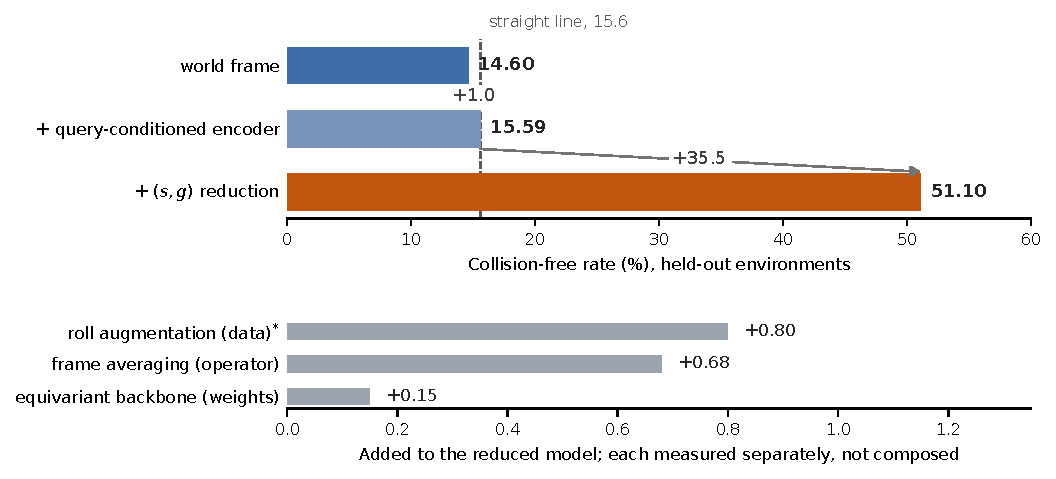
\includegraphics[width=\columnwidth]{fig_cascade.pdf}
\caption{Lorem ipsum dolor sit amet, consectetur adipiscing elit sed do
eiusmod tempor incididunt ut labore}
\label{fig:teaser}
\end{figure}

% ============================== PAGE 2 (1.0) =========================
\section{Related Work}
% ~250 words. Three clusters, roughly 80 words each: equivariant
% architectures; canonicalisation and frame averaging; generative planners.
\filler{9}

\section{Method}
\subsection{Decomposing the group}
% ~200 words plus the two propositions.
\filler{7}

\begin{proposition}[Lorem ipsum]
\label{prop:one}
Lorem ipsum dolor sit amet, consectetur adipiscing elit, sed do eiusmod tempor
incididunt ut labore et dolore magna aliqua $X' = R_{\hat{x}}(\theta)\,X$.
\end{proposition}

\begin{proposition}[Dolor sit amet]
\label{prop:two}
Lorem ipsum dolor sit amet consectetur adipiscing elit sed do eiusmod tempor
incididunt ut labore.
\end{proposition}
% Two-line proof only. Anything longer goes in an appendix or is cut.
\begin{proof}
Lorem ipsum dolor sit amet consectetur adipiscing elit, sed do eiusmod tempor
incididunt ut labore et dolore magna aliqua ut enim ad minim veniam.
\end{proof}

% ============================== PAGES 3--4 (1.2) =====================
\section{Setup and Calibration}
\subsection{Benchmark and protocol}
% ~180 words. Workspace, obstacle counts, trajectory length, held-out split,
% sample count, integrator budget. Dense and factual; no argument here.
\filler{5}

\begin{table}[t]
\centering
\footnotesize
\setlength{\tabcolsep}{3.5pt}
\begin{tabular}{@{}lrrr@{}}
\toprule
Lorem & Ipsum (\%) & Dolor & s/query \\
\midrule
lorem ipsum          & 00.0 & 0.000 & $<$0.001 \\
dolor sit            & 00.0 & 0.000 & 0.000 \\
amet consectetur     & 00.0 & 0.000 & 0.000 \\
adipiscing elit      & 00.0 & 0.000 & 0.000 \\
sed do eiusmod       & 00.0 & 0.000 & 0.000 \\
\midrule
tempor incididunt    & 00.0 & $-$0.000 & 0.000 \\
ut labore et dolore  & \textbf{00.0} & $-$0.000 & 0.000 \\
\bottomrule
\end{tabular}
\caption{Lorem ipsum dolor sit amet consectetur adipiscing elit sed do eiusmod
tempor incididunt ut labore et dolore magna aliqua}
\label{tab:floors}
\end{table}

\subsection{The floor, and a paired test against it}
% ~200 words. The trivial baseline, the arm that does not beat it, and WHY the
% test is paired rather than a comparison of two independently resampled rates.
\filler{7}

% ============================== PAGES 4--5 (1.3) =====================
\section{Results}
\subsection{Scaling}
% ~220 words.
\filler{7}

\begin{figure}[t]
\centering
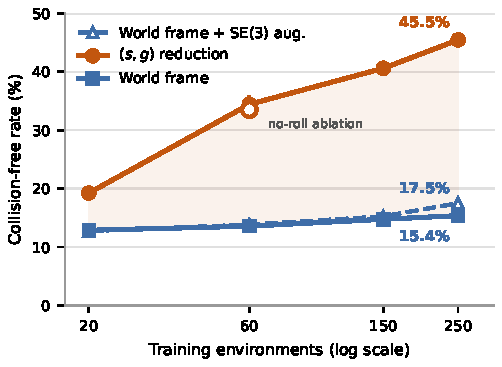
\includegraphics[width=\columnwidth]{fig_scaling_col.pdf}
\caption{Lorem ipsum dolor sit amet consectetur adipiscing elit}
\label{fig:scaling}
\end{figure}

\begin{table}[t]
\centering
\footnotesize
\setlength{\tabcolsep}{3.5pt}
% MERGED mechanism table: one row per mechanism, one column per budget.
\begin{tabular}{@{}l r r >{\raggedright\arraybackslash}p{1.7cm}@{}}
\toprule
Lorem ipsum & A & B & Dolor \\
\midrule
lorem ipsum dolor      & $+00.0$ & $+00.0$ & sit amet \\
\quad consectetur      & $+00.0$ & ---     & adipiscing \\
\quad elit sed         & $+00.0$ & ---     & eiusmod \\
tempor incididunt      & $+0.0$  & ---     & ut labore \\
et dolore magna        & $+0.0$  & $+0.00$ & aliqua \\
ut enim ad minim       & ---     & $+0.00$ & veniam quis \\
\bottomrule
\end{tabular}
\caption{Lorem ipsum dolor sit amet consectetur adipiscing elit sed do eiusmod}
\label{tab:mechanisms}
\end{table}

\begin{figure}[t]
\centering
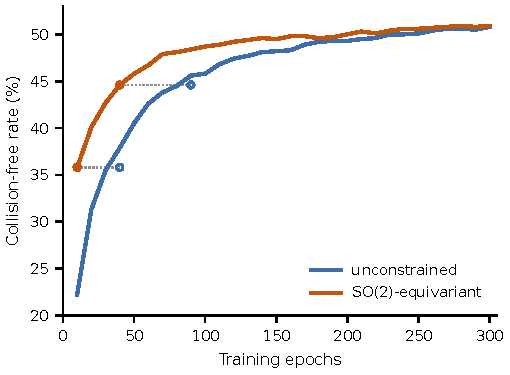
\includegraphics[width=\columnwidth]{fig_convergence.pdf}
\caption{Lorem ipsum dolor sit amet consectetur adipiscing}
\label{fig:conv}
\end{figure}

% ============================== PAGES 5--6 (1.2) =====================
\subsection{Control: a query-conditioned encoder}
% ~250 words. State the deflationary objection in its STRONGEST form first,
% then the arm built to test it, then the number.
\filler{9}

\subsection{Control: local geometry, and how it scales}
% ~300 words. The 2x2, the value that survives, the honest ordering, and the
% decay at matched budget.
\filler{9}

\begin{table}[t]
\centering
\footnotesize
\setlength{\tabcolsep}{3.5pt}
\begin{tabular}{@{}lrrr@{}}
\toprule
Lorem ipsum & Dolor & Sit & $\Delta$ \\
\midrule
lorem ipsum       & 00.00 & 00.00 & $+00.0$ \\
dolor sit amet    & 00.00 & 00.00 & $+00.0$ \\
\quad consectetur & 00.00 & \textbf{00.00} & $+00.0$ \\
\midrule
\emph{adipiscing} & $+00.0$ & $+00.0$ & \\
\bottomrule
\end{tabular}
\caption{Lorem ipsum dolor sit amet consectetur adipiscing elit sed do eiusmod
tempor incididunt}
\label{tab:twobytwo}
\end{table}

% ============================== PAGE 6--7 (0.8) ======================
\subsection{Replications}
% ~180 words covering all three at once. One table, three blocks of rows.
\filler{5}

\begin{table}[t]
\centering
\footnotesize
\setlength{\tabcolsep}{3.5pt}
\begin{tabular}{@{}llrrr@{}}
\toprule
Lorem & Ipsum & A & B & $\Delta$ \\
\midrule
dolor   & sit amet     & 00.0 & 00.0 & $+00.0$ \\
        & consectetur  & 00.0 & 00.0 & $+00.0$ \\
\midrule
elit    & sed do       & 00.0 & 00.0 & $+00.0$ \\
        & eiusmod      & 00.0 & 00.0 & $+00.0$ \\
\midrule
tempor  & incididunt   & 00.0 & 00.0 & $+00.0$ \\
        & ut labore    & 00.0 & 00.0 & $+00.0$ \\
\bottomrule
\end{tabular}
\caption{Lorem ipsum dolor sit amet consectetur adipiscing elit}
\label{tab:replications}
\end{table}

\subsection{The residual, and what it bounds}
% A THIRD OF A COLUMN. ~120 words plus the corollary. State the bound, state
% that it does not predict, cite the prior work for the projection property,
% and stop.
\filler{4}

\begin{corollary}[Lorem ipsum]
\label{cor:budget}
Lorem ipsum dolor sit amet consectetur adipiscing elit, sed do eiusmod tempor
incididunt $\|f - \mathcal{A}f\|^2 \le r^2$.
\end{corollary}

% ============================== PAGE 7 (0.8) =========================
\section{Limitations}
% ~200 words. Scope condition first, then seeds, then the single benchmark
% family. Keep the self-corrections: they cost little and buy credibility.
\filler{7}

\section{Conclusion}
% ~120 words. Shorter than feels comfortable.
\filler{4}

% ============================== (0.7) ================================
\small
\begin{thebibliography}{99}
\bibitem{lorem} Lorem Ipsum and Dolor Sit.
\newblock Consectetur adipiscing elit sed do eiusmod.
\newblock {\em Tempor Incididunt}, 2024.
\bibitem{ipsum} Amet Consectetur.
\newblock Ut labore et dolore magna aliqua.
\newblock In {\em Proc. Ut Enim Ad Minim}, 2023.
\end{thebibliography}

\end{document}
